\appendix

\chapter{Notes}

\section{Mixins help reduce sharing constraints}
\label{sec:mixins-reduce-sharing-constraints}

The goal of this appendix is to explain why mixins help ``avoid the
preponderance of sharing constraints that occur with ML functors.''
(as claimed in Section~\ref{sec:intro})  For concreteness, the ML
examples in this section will be written in OCaml.

\paragraph{What is a sharing constraint?}
Ordinarily, an abstract type in a signature is not equal to any other type.  A
sharing constraint \verb|with type t = u| asks the compiler to expose
the fact that the abstract type \verb|t| is equal to some other type \verb|u|.%
\footnote{For the language lawyers out there, SML also defined a
construct \texttt{sharing type} which is a specialized signature
refinement operator for specifying that two abstract type components
inside a signature are transparently equal (the \texttt{with type} construct
doesn't suffice for this case, since an abstract type defined inside
the signature is not a valid type outside the signature.) We'll use
the colloquial meaning of sharing constraints to refer to both constructs.}
In ML, sharing constraints are needed most commonly in two situations:

\begin{enumerate}
    \item When a module is \emph{sealed} by some signature, a sharing
    constraint may be used to reveal some types which would otherwise
    be opaque. For example, consider these modules for maps with arbitrary
    keys:

\begin{lstlisting}[language=ML]
        module IntMap =
          struct
            type key = int
            type 'a t = ...
            let insert k v m = ...
          end
        module type MAP =
          sig
            type key
            type 'a t
            val insert : key -> 'a -> 'a t -> 'a t
          end
        module SealedIntMap = (IntMap : MAP)
\end{lstlisting}

    \noindent In this example, the resulting \verb|SealedIntMap| has
    an opaque \verb|key| and \verb|t| type, because it was sealed
    with the signature for \verb|MAP|.  However, there is a problem
    with \verb|SealedIntMap|: we don't
    know anything about the type of \verb|key|, and thus cannot actually
    use \verb|insert| (because we can't produce a value of type \verb|key|).

    A sharing constraint allows us to add a constraint to the signature \verb|MAP|
    saying, ``And actually, \verb|key| is an \verb|int|'':

\begin{lstlisting}
    module BetterSealedIntMap = (IntMap : MAP with type key = int)
\end{lstlisting}

    \noindent We won't say much about this use case, because \Backpack{} does
    not support sealing, so there isn't a point of comparison.

    \item A sharing constraint may be used to relate types between multiple
    signatures, which specify arguments to a functor.  For example:

\begin{lstlisting}[language=ML,escapechar=@]
    module type A = sig type t;; val f : t -> t end
    module type B = sig type t;; val g : t      end
    module F (X : A) (Y : B with type t = X.t) = struct let z = @\fbox{X.f Y.g}@ end
\end{lstlisting}

    Here, \verb|X.t| and \verb|Y.t| are not type equal without the
    sharing constraint \verb|with type t = X.T| on \verb|B|; without
    the sharing constraint, the boxed \verb|X.f Y.g| would not typecheck.

\end{enumerate}

\noindent
In fact, \Backpack{} also supports sharing constraints: for example,
if an inherited signature defines an abstract type \verb|data T|, we
can define a local signature at this name with the declaration \verb|type T = Int|
to refine the abstract type \verb|T| into \verb|Int|.

\paragraph{How does Backpack eliminate sharing constraints?}  In a mixin
module system like \Backpack{}, a sharing constraint is implicitly generated
whenever two types are brought into scope under the same name.  For example,
if I depend on two packages which both require an implementation of
\verb|Str|, the two signatures will be merged together, so that \verb|Str|
from the signature of the first package and \verb|Str| from the signature
of the second package are treated as the same type.

An analogous situation in ML occurs when I have two functors,
which I would like to instantiate with the same module:

\begin{lstlisting}[language=ML,escapechar=@]
    module type A1 = sig type t;; val f : t -> t end
    module type A2 = sig type t;; val g : t      end
    module F1 (X : A1) = struct ... end
    module F2 (X : A2) = struct ... end
    module F (X : @\fbox{???}@) = struct
        module M1 = F1(X)
        module M2 = F2(X)
        ...
    end
\end{lstlisting}

\noindent
What signature can we can we give here?  Unlike in \Backpack{}, we must
specify the signature.  One possibility is to write the merged signature
by hand:

\begin{lstlisting}[language=ML,escapechar=@]
    module type A =
      sig type t
          val f : t -> t
          val g : t
      end
\end{lstlisting}

\noindent
This may be tiresome if the signatures are large.  Fortunately,
ML also supports the \verb|include| construct, which textually includes
the contents of a signature into a new signature, which can be used to
construct the merged signature by including both signatures.  However, there is a twist:

\begin{lstlisting}[language=ML,escapechar=@]
    module type A =
      sig include A1
          include A2 with t := t
      end
\end{lstlisting}

\noindent
We must relate the \verb|t| from \verb|A1| with the type \verb|t| from
\verb|A2|. In OCaml, we can
declare this relationship with a \emph{destructive substitution}.
The destructive substitution \verb|type t := t| says, ``Find all occurrences
of \verb|t| inside \verb|A2|, replace them with the \verb|t| that is in
scope (from \verb|A1|), and delete \verb|type t| from \verb|A2|.''
The final signature is equivalent to the one we wrote out by hand.

Destructive substitution only works for types, so if two signatures
define the same functions or values, your only recourse is to write the
merged signature by hand, or pass in two modules, one for each signature,
with the necessary sharing constraints to witness the necessary type equalities
(as seen in the example functor with two module arguments).

\paragraph{Summary}
\Backpack{} doesn't eliminate all cases where sharing constraints might be
useful; for example, a user of \Backpack{} may still find it useful to
declare \verb|type Key = Int| to refine the type of an abstract map
to be a map with integer keys.  However, it does eliminate one important
class of sharing constraints which arise when there are multiple signatures
describing the same types and functions.

%   \begin{tabular}{p{0.45\textwidth} p{0.45\textwidth}}
%   \begin{lstlisting}[language=ML]
%   module type A1 = sig
%       type t = int
%       type u
%       val f : int -> u
%   end
%   \end{lstlisting}
%   &
%   \begin{lstlisting}[language=ML]
%   module type A2 = sig
%       type t
%       type u = bool
%       val f : t -> bool
%   end
%   \end{lstlisting}
%   \end{tabular}


%   Sharing constraints in ML permit users to specify that two modules
%   specify the same abstract type.
%   Here is an example application of
%   sharing constraints in OCaml adapted from the OCaml FAQ\footnote{\url{https://caml.inria.fr/resources/doc/faq/module.en.html}}:
%   \begin{lstlisting}[language=ML,escapechar=@]
%       module type S1 = sig type t
%                            val x : t
%                        end
%       module type S2 = sig type t
%                            val f : t -> t
%                        end
%       module F (X : S1) (Y : S2 with type t = X.t) =
%         struct
%           let g = Y.f X.x
%         end
%   \end{lstlisting}
%   %
%   In this example, the signatures \verb|S1| and \verb|S2| both define
%   an abstract type \verb|t| and some values which operate on this type.
%   When we define a functor \verb|F| which takes a module of type \verb|S1|
%   and a module of type \verb|S2|, it is \emph{not} automatically the case
%   that the \verb|t| from \verb|X| and the \verb|t| from \verb|Y| are the same.
%   To declare that these types are the same, we specify a sharing constraint
%   \verb|with type t = X.t| which declares the equality between \verb|X.t|
%   and \verb|Y.t|.

\chapter{Recursive linking}
\label{sec:recursive-linking}

In this section, we sketch how to add support for recursive linking to
\Backpack{}, allowing us to mix-in link libraries which recursively
depend on each other.  Even though \Backpack{} as described in this
thesis does not support recursive linking, many aspects of its design
(e.g., mix-ins) were inherited from systems which did support recursive
linking (notably, \OldBackpack{} and MixML).

%   We will first informally describe how to make use of recursive
%   linking in \Backpack{}, pointing out some subtleties that arise
%   in the presence of recursive linking.  Then we will sketch semantics
%   for recursive linking, and 

\section{A simple example}

Suppose that you have modules implementing logging and database access,
with the following interfaces:

\begin{lstlisting}
    signature Logging where
        data LogHandle
        log :: LogHandle -> String -> IO ()

    signature Database where
        data DbHandle
        data Query a
        query :: DbHandle -> Query a -> IO a
\end{lstlisting}
%
A cyclic dependency may arise if the database service logs queries with
the logging API, but you have a database-backed logger which is
implemented using the database API\@.\footnote{Let us not consider the
wisdom of logging to a database or structuring the API this way.}  In
conventional Haskell, we can place these in separate modules and break
the cyclic imports with an \verb|hs-boot| file:

\begin{lstlisting}
    -- Database.hs-boot
    module Database where
        data DbHandle
        data Query a
        query :: DbHandle -> Query a -> IO a

    -- Logging.hs
    module Logging where
        import {-# SOURCE #-} Database
        data LogHandle = ...
        log :: LogHandle -> String -> IO ()
        log = ...

    -- Database.hs
    module Database where
        import Logging
        data DbHandle = ...
        data Query a = ...
        query :: DbHandle -> Query a -> IO a
        query = ...
\end{lstlisting}
%
If you want to place \verb|Database| and \verb|Logging| in separate
packages, \verb|hs-boot| files are insufficient---\Backpack{} with
recursive linking, however, will get the job done:

\begin{lstlisting}[language=Cabal]
    -- database.cabal
    name: database
    library
      exposed-modules: Database
      signatures: Logging

    -- logging.cabal
    name: logging
    library
      exposed-modules: Logging
      signatures: Database
\end{lstlisting}
%
If a package depends on both \verb|database| and \verb|logging|,
\verb|database|'s \verb|Logging| requirement will be filled with \verb|logging|,
and vice versa.  Alternately, \verb|database| can have a direct
dependency on \verb|logging|, filling \verb|logging|'s requirement with a module
it defines locally.

\begin{lstlisting}[language=Cabal]
    -- logging.cabal as before

    -- database.cabal
    name: database
    library
      build-depends: logging
      exposed-modules: Database
\end{lstlisting}

\paragraph{Comparison with \OldBackpack{}}
In \OldBackpack{}, signatures subsume \verb|hs-boot| files, because a signature
and a module can be defined in the same package:

\begin{lstlisting}
    package p where
        Database :: [ ... ]
        Logging  = [ import Database; ... ]
        Database = [ import Logging; ... ]
\end{lstlisting}
%
Although we briefly attempted to implement this design, we eventually
decided to keep \verb|hs-boot| and \verb|hsig| files as distinct
concepts.  The big problem is that \OldBackpack{} assumes an explicit
user-specified ordering on the modules and signatures in a package,
while Haskell code written in the wild today assumes an implicit
ordering specified by the import statements in modules.  There is no
convenient way to specify how a module and its signature should be
ordered relative to other modules, without adopting an \verb|hs-boot|
style \verb|{-# SOURCE #-}| import syntax.

\section{Challenges}

The presence of recursive linking introduces new complications for
type checking.

\paragraph{Cyclic exports}  Consider the following recursive module
definition:

\begin{lstlisting}
    -- package b
    signature A where
        x :: Int
    module B(x) where
        import A(x)
    -- package a, which depends on b
    module A(x) where
        import B(x)
\end{lstlisting}

In Haskell, an implementation cycle isn't necessarily a problem,
because a binding like \verb|x = x| can simply be compiled into a thunk
which infinite loops when forced.  However, what should be the original
name of this \verb|x|?  There is no appropriate name, because there
isn't any module (not signature) which ever defines \verb|x|.  Thus,
recursive \Backpack{} must reject this implementation.

(\verb|hs-boot| files do not suffer from this problem, because GHC
Haskell does not permit entities in an \verb|hs-boot| file to be implemented
using a reexport.)

\paragraph{No backwards propagation}
GHC is an incremental compiler: if you edit a module of a previously
compiled project, only modules which transitively import it need to be
recompiled.  For this strategy to be correct, it must not be the case
that a downstream module can affect the compilation of an upstream one.
Unfortunately, the \emph{shaping pass} of \OldBackpack{}---used to
prevent the double vision problem---is a pre-pass
which can cause information to propagate backwards.  Consider the
following example:

\begin{lstlisting}[escapechar=@]
    package p where
        A :: [ data T ]
        B = [ import A; f (x :: T) = x ]
    package q where
        include p
        I = [ data T = MkT ]
        C = [ import B; import I; y = @\fbox{f MkT}@ ]
        A = [ exports (T); import C; import I(T) ]
\end{lstlisting}
%
Here, the shaping pass determines that the abstract \verb|T| from
\verb|A| and the concrete \verb|T| from \verb|I| coincide, ensuring that
the enboxed \verb|f MkT| will typecheck.  We can see that if we
modify the implementation of \verb|A| (last line) to define a different
\verb|T|, this equality would no longer hold, and \verb|C| would
fail to typecheck.  Thus, information propagates backwards from
the implementation of \verb|A| to \verb|C|.

In \Backpack{}, we propose that \verb|f MkT| should \emph{not}
typecheck, in order to preserve incremental compilation.  More
generally, only the implementor of a module and any modules which
transitively import it should be affected by any refinements to original
names that occur due to exports in the implementation of a module.
Consequently, we refine the original names of a forward reference only
immediately before we typecheck the implementation of this forward
reference.

%   Lack of backwards propagation also causes a technical difficulty in
%   implementation: after type checking modules, we may need to write out
%   references to as yet to be resolved hole variables (which will later be
%   recursively defined), on faith that they will be backpatched to the
%   correctly values later.

%   This change also allows us to sidestep some infelicities with
%   \OldBackpack{}'s shaping pass:

%   \begin{lstlisting}[escapechar=@]
%       package p where
%           A :: [ data T ]
%           B = [ exports (T); import A ]
%       package q where
%           include p
%           I = [ data T = MkT ]
%           C = [ @\fbox{exports (T)}@; import B; import I ]
%           A = [ exports (T); import I(T) ]
%   \end{lstlisting}

%   Under \OldBackpack{}'s backwards propagating semantics,
%   we might say that \verb|C|'s export of \verb|T|
%   is unambiguous (because of the implementation of \verb|A|).
%   However, \OldBackpack{} will reject \verb|C| during
%   shaping, because at the time of shaping, we must resolve the export of
%   \verb|T|, but it is not known that \verb|I.T| and \verb|B.T| coincide
%   (that's what shaping is trying to figure out!)  In principle, this
%   problem could be solved by a more sophisticated shaping algorithm,
%   but this is 

\paragraph{Translucency}  A feature not supported in \OldBackpack{}
but supported in \Backpack{} is
the ability to use a type synonym to implement an abstract data type.
This introduces a form of ``translucency'', where the abstract data type
is opaque while the implementation is unknown, and transparent afterwards.
For example, in Section~\ref{sec:instantiating-the-matcher}, we demonstrated
how we could instantiate a generic regular expression matcher to match on strings.
Inside the implementation of the matcher, we knew nothing about the abstract
type \verb|Str|; after instantiating it, the \verb|accept| function
transparently accepts \verb|String| arguments.

Translucency introduces yet another variant of the \emph{double vision}
problem.  In systems like RMC and MixML, double vision is solved by
introducing a type precomputation pass, which means that we end up
with same kind of backwards propagation we described in \OldBackpack{}.
Here is the analogous example, rewritten to use translucency rather than
exports:

\begin{lstlisting}[escapechar=@]
    -- package p
    signature A where
        data T
    module B where
        import A
        f (x :: T) = x
    -- package q, which depends on p
    module C where
        import B
        y = @\fbox{f 2}@
    module A where
        import C
        type T = Int
\end{lstlisting}
%
Here, we provide a forward declaration of \verb|A| which
declares \verb|T| abstractly, which is eventually declared to be
a type synonym of \verb|Int|.  The key expression is boxed: does \verb|f 2|
in module \verb|C| typecheck?

Just as we argued previously, we think \verb|f 2| should \emph{not}
typecheck.  If we were to move the definition of \verb|y| to \verb|A|
(or any module that imports \verb|A|) it should typecheck in all cases.
This is in contrast to the behavior of MixML\@:

\begin{figure}[H]
\begin{tabular}{p{0.40\textwidth} p{0.50\textwidth}}
\begin{lstlisting}[language=ML,escapechar=@]
link X = { type t }
with ( { val f (x : X.t) = x,
         val y = @\fbox{f 2}@ }
           with
       { type t = int } )
\end{lstlisting}
&
\begin{verbatim}
(* mixml 0.2.1 passes with type: *)
it : {f : [int -> int]+,
      t : [= int : #],
      y : [int]+}
\end{verbatim}
\end{tabular}
\caption{Backwards propagating type information in MixML}
\label{fig:double-vision-backwards-propagating-mixml}
\end{figure}

\noindent
Although we have very loosely translated the example (a more
faithful example would actually construct \verb|f|, \verb|y| and
\verb|t| in substructures representing each Haskell level
module), the same basic pattern holds: when typechecking \verb|f 2|,
\verb|X.t| is already known to be equal to \verb|int|.

\section{Recursive \uid{}s}
\label{sec:recursive-uids}

%   **Warning:** The extension described in this section is not implemented
%   in GHC 8.2.  It can be skipped upon a first reading.

\Backpack{} with recursive linking requires generalizing unit
identifiers to be infinite regular trees.  As was the case
in \OldBackpack{}, these trees can be
represently finitely using $\mu$-binders (ala recursive types),
with the following abstract syntax (where $\alpha$ ranges over
unit identity variables):

\[
\begin{array}{rcll}
  \UP &::=& \mu\alpha.\, \icid{\Up}{S} & \text{\Uid} \\
      & | & \alpha \\
\end{array}
\]

%   A more parsimonious extension to the concrete syntax is to
%   have every ``ComponentId`` "constructor" implicitly introduce
%   a μ-binding, and represent the variables with de Bruijn indexes.
%   Let ``UnitIdVar`` range over natural numbers, then:

%   ::

%       UnitId ::= ComponentId "[" ModuleSubst "]"
%                | UnitIdVar

Pictorially, recursive components simply relax the acyclicity restriction on
the component graph:

\begin{figure}[H]
\center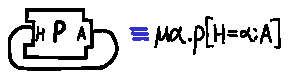
\includegraphics{figures/recursive-unit-identifier.pdf}
\end{figure}

These graphs are equivalent up to unfoldings (i.e., unrolling the
cycles).
As observed in \OldBackpack{}, infinite trees of this form
can be tested for equivalence using Huet's unification algorithm.
However, for an implementation, it is more convenient to compute the canonical form
of a \uid{}, so equality can be checked syntactically.  This can be
computed by Moore machine minimization.  Canonicalization can be achieved
in three steps:

\begin{enumerate}
\item Convert the unit identifier into a Moore machine,
\item Minimize the Moore machine (the procedure is similar to DFA
   minimization, except that states with differing outputs are
   initialized to be in separate equivalence classes initially), and
\item Convert the Moore machine back into a unit identifier.
\end{enumerate}
%
Intuitively, the Moore machine of a unit identifier recognizes paths
(from right to left) through the component graph, outputting the
component identifiers of the component boxes it traverses.

\begin{figure}[H]
\center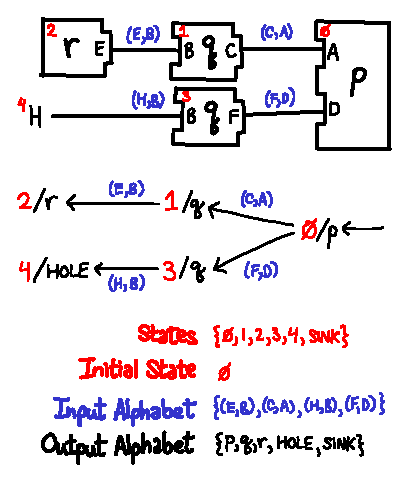
\includegraphics{figures/moore-description.pdf}
\end{figure}

\noindent
Formally, we define the partial Moore machine corresponding to a unit
identifier as follows:

\begin{enumerate}
\item The state set ranges over component boxes and hole modules in the
   graph (in the diagram above, we simply assigned a number to each
   box/hole).
\item The input alphabet is the Cartesian product of output module names
   and input module names.  Intuitively, each member of the alphabet
   corresponds to a wire labeled with the name of the input and output
   ports it is wired to.
\item The output alphabet is the set of component identifiers, as well
   as a distinguished element \verb|HOLE| for hole modules.
\item The inital state is the state corresponding to the component box of
   the unit identifier we want to denote.
\item A transition from $q$ to $q'$ on the input $(m, m')$ exists
   if there is a wire from the input port $m'$ of $q$ to the output
   port $m$ of $q'$ (or a hole module $\hv{m}$, if $q'$ corresponds to a hole
   module).
\item The output of a state is the component identifier of its component
   box, or \verb|HOLE| if it is a hole module.
\end{enumerate}
%
We can complete the partial Moore machine into a total Moore machine by
adding a new sink state \verb|SINK|, which outputs a new output value
\verb|SINK|, and directing all undefined transitions to it (not depicted on
the diagram).

Here are two examples of recursive components expressed as Moore
machines:

\begin{figure}[H]
\center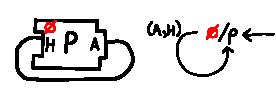
\includegraphics{figures/moore-p.pdf}
\hspace{3em}
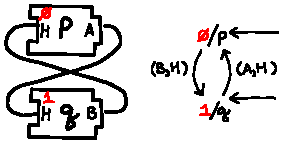
\includegraphics{figures/moore-pq.pdf}
\end{figure}

\noindent
The \uid{} corresponding to a Moore machine is defined by
recursively traversing the Moore machine, creating unit identifiers
whose component identifier is the output at a state, and module
substitution is all of the outgoing transitions to non-sink states. During
this traversal, we maintain a stack of seen states:  when we reach a
state that is already on our stack, we emit a variable bound
for that state on the stack.  This traversal
is guaranteed to terminate as the size of the state set is finite.

\section{Mix-in linking}

Mix-in linking can be straightforwardly adapted to a recursive
setting: the algorithm proceeds as before, but we remove the
occurs check from unification, allowing our unification to
produce infinite trees (as describe above.)  Pictorially,
this simply corresponds to allowing loops when we wire up provisions
to requirements in our component shapes.

\section{Type checking}

The primary complexity of handling recursive linking during type
checking comes down to handling the double vision problem.  To avoid
double vision, typechecking rules must be organized so that the
types/identities of a forward declaration are not used until we finish
computing them.  \OldBackpack{}, MixML and RMC engineer this by
literally separating out this computation as a separate pre-pass.  In
this sketch of recursive linking for \Backpack{}, we'll take a different
approach, taking advantage of the natural staging that occurs in Haskell
typechecking to achieve a similar effect.

\paragraph{Type lookup}
Before we discuss renaming and typechecking for Haskell proper,
it is worth describing how the presence of recursive unit identifiers
affects the type lookup process.  Suppose we're the type of
$\mu\alpha.\, \Mod{\icid{p}{ \subst{A}{\Mod{\alpha}{M}} }}{M}$.
Naively, if we recursively lookup the module types of the modules
in this substitution, so as to construct the required name
substitution, we will suffer from infinite regress.

Fortunately, matters are different if we \emph{lazily} lookup the
original name of a name hole post substitution.  In this situation,
if the original name is well-defined, we will eventually bottom out
with the correct answer.  To detect if an infinite loop has occurred,
we can simply keep track of module identities which we are performing
this lookup for: if a module recurs, we know that we are in an
infinite loop.

Here is a particularly complicated example which demonstrates this
principle:

\begin{lstlisting}
    module A where
        data T = MkT
    signature B where
        data T
    module C(T) where
        import B(T)
    signature D where
        data T
    module E(T) where
        import D(T)
\end{lstlisting}

Suppose this we recursively instantiate this package as per the
following wiring diagram (call this unit identifier $P$):

\begin{figure}[H]
\center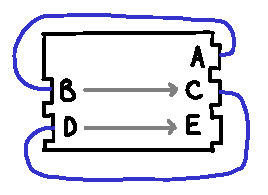
\includegraphics{figures/recursive-uid-example.pdf}
\end{figure}

Suppose we want to look up the original name of the export \verb|T| from
$\Mod{P}{E}$.  We can see in the interface of \verb|D| that,
uninstantiated, \verb|E| exports $\nhv{D.T}$.  By the substitution, this
means we must lookup $\Mod{P}{C}$.  Once again, uninstantiated, \verb|C|
exports $\nhv{B.T}$.  By the substitution, we lookup $\Mod{P}{A}$ and
finally get the true original name of \verb|T|.  If instead \verb|B| was
instantiated with $\Mod{P}{C}$, we would once again lookup $\Mod{P}{C}$
and bail out, as we have discovered an infinite loop.

\paragraph{Renaming}
During renaming, it is necessary to look up the export specifications of
modules we have imported in order to compute the original names of any
reexported entities.  Thus, the key cases in a recursive setting are
handling cases when we are required to look up the export specification
of the module/signature we are currently renaming, or possibly even an
export of a local module/signature which transitively imports the
current module/signature.

In the first case, matters are relatively simple: in a well-typed
module/signature, it is impossible to reexport a forward reference of
this very module/signature, as that would immediately result in a cycle
(reexports cannot rename, and there is always a unique export for any
occurrence name.)

In the second case, there is no way to lookup the export specification
of the local module/signature in question, as it would be a violation of the
no backwards propagation principle to look at the source.  Instead, we
lookup the merged export specification of our dependencies (sans the local
module/signature.)  When the local module/signature is finally typechecked,
we simply need to update the identities in question.

\paragraph{Typechecking}
Handling recursive linking in type checking is easier than with
renaming, because GHC Haskell is already equipped to handle mutually
recursive type definitions within a single module.  In Haskell typechecking,
we first kind-check all type declarations and add them to the environment
(applying any updated definitions to the context), before typechecking
any value declarations.  This means that we never typecheck a value
declaration (the only situation where type-based double vision can
occur) before we have computed the types of all forward declared type
declarations.  One minor complication, as in the renaming case, is that
if we attempt to lookup a type which is not locally defined (either
because it was inherited from a signature, or it comes from a module/signature
which transitively imports us), we should instead defer to the type
from the merge of only the dependencies.

One final remark: one reason why handling double vision in Haskell is so
simple is because we have no mechanism for post-facto \emph{sealing}, unlike
many ML module systems.  Without sealing, we can always compute the types
first, and then handle the values.  With sealing, things are far more complicated:
you must be able to vary which types are transparent and which are opaque when your
have sealed mutually recursive modules.

